\definecolor{customBlue}{HTML}{27aeef} % Hex code for DodgerBlue
\definecolor{customGreen}{HTML}{87bc45} % Hex code for Tomato
\definecolor{customYellow}{HTML}{ede15b} % Hex code for Gold
\definecolor{customOrange}{HTML}{ef9b20}

\section{Úvod}
Tato práce je zpracována jako projekt do předmětu Modelování a simulace. Vybraným tématem projektu je T2: SHO Model výroby v oblasti potravinářství, kde jsme se konkrétně zaměřili na simulaci výrobní linky bramborových chipsů. Cílem této práce je vytvoření detailního modelu celé výrobní linky, zohledňující všechny procesy a postupy při výrobě bramborových chipsů a následné experimentování s jednotlivými parametry výrobní linky a procesů pro získání nových poznatků, které povedou k optimalizaci výrobního procesu.

\paragraph{Počáteční otázka}
TODO: Jak můžou změny parametrů výrobní linky či změny procesů optimalizovat efektivitu výroby?\\

\newpage
\section{Petriho síť}
\begin{figure}[h!]
    \centering
    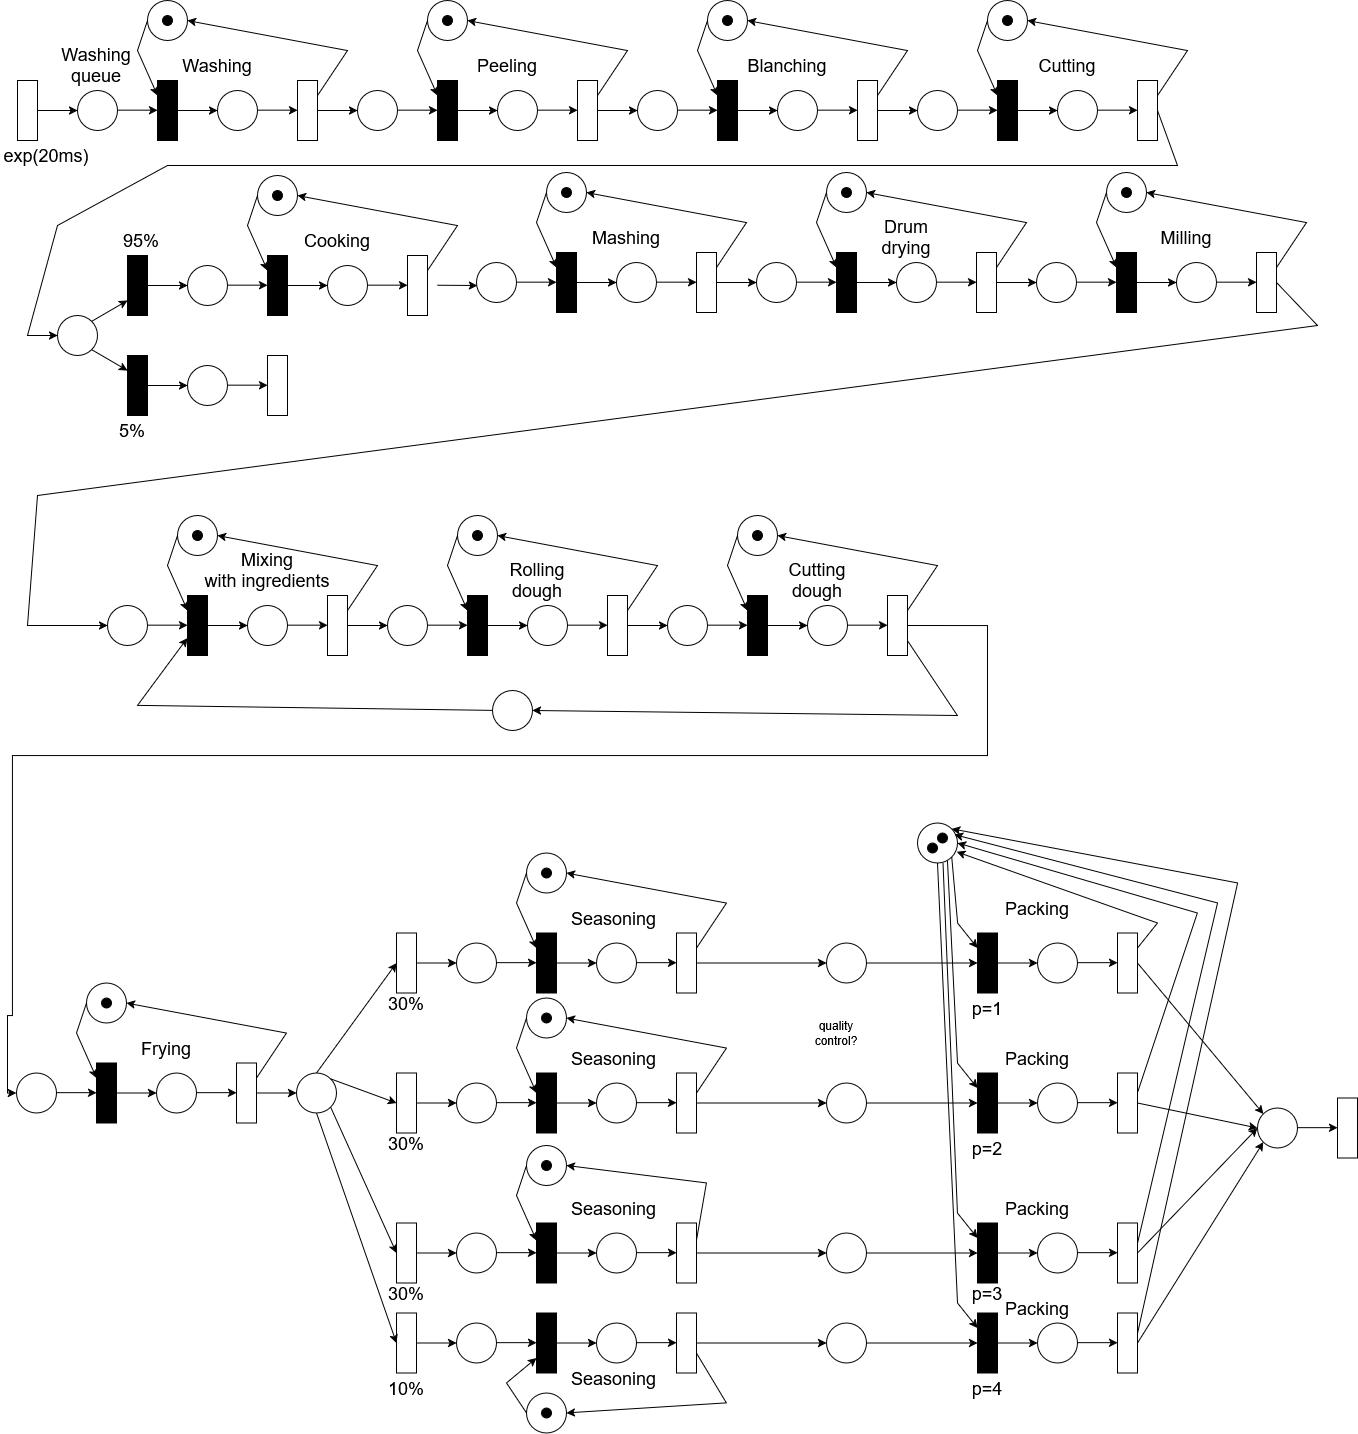
\includegraphics[width=\textwidth]{fig/IMS Pringles3.drawio.png}
    \caption{Petriho síť výrobního procesu}
    \label{Petriho síť výrobního procesu}
\end{figure}